\documentclass[12pt,a4paper]{article}

% Margins.
\setlength{\oddsidemargin}{0in}
\setlength{\evensidemargin}{0in}
\setlength{\headheight}{12pt}
\setlength{\headsep}{42pt}
\setlength{\topmargin}{-54pt}
\setlength{\textwidth}{6.5in}
\setlength{\textheight}{10in}

\usepackage{amsmath}
\usepackage{float}
\usepackage{graphicx}
\usepackage[hyphens]{url}
\usepackage{hyperref}	% Clickable links to figures, references and urls.
\usepackage{datetime}
\usepackage{longtable}

% Links direct to top of figures.
\usepackage[all]{hypcap}

% Drawing.
\usepackage{pgf}
\usepackage{tikz}

% Listings for formatting code.
\usepackage{listings}
\usepackage{textcomp}
% General options.
\lstset{breaklines=true, basicstyle=\small\ttfamily, tabsize=4, numbers=left, stepnumber=1, frame=single, showstringspaces=false, upquote=true}
% C++ specific high-lighting. Comments are 50/50 shades of green/black and strings coloured with 60/40 red/black mixture.
\lstset{language=[ISO]C++, commentstyle=\color{green!50!black}, keywordstyle=\color{blue}, stringstyle=\color{red!60!black}}

%opening
\title{\vspace{-2cm}Physics for Engineers\\Class 07\\Constant Coordinate Surfaces}
\author{Attique Dawood}
\date{September 02, 2013\\[0.2cm] Last Modified: \today, \currenttime}
\begin{document}
\maketitle
\section{Announcements}
\begin{itemize}
\item Assignment \#01 is due Today
\item Quiz \#02 today.
\end{itemize}
\section{Revision}
\begin{itemize}
\item Cartesian, cylindrical and spherical coordinate systems.
\end{itemize}
\section{Orientation of Unit Vectors in Coordinate Systems}
In Cartesian coordinates the unit vectors $\hat x$, $\hat y$ and $\hat z$ are constant and have a fixed direction at each point in the whole space.

In Cylindrical coordinate system, $\hat \rho$ and $\hat \phi$ have different directions depending on location. Pick a point, direction of $\hat \rho$ is radially outward from the $z$--axis at that point. Similarly, direction of $\hat \phi$ is increasing direction of $\phi$. Direction of $\hat \phi$ is tangent to a circle drawn at the given point with $\hat \rho$ pointing outward along the radial segment. Note that all three unit vectors are mutually perpendicular at each point in the whole space.
\section{Constant Coordinate Surfaces (2.5S)}
\subsection{Cartesian Coordinates}
If we let $z=0$ and let $x$ and $y$ vary then we get a set of points known as the $xy$--plane. This is also called the $z=0$ plane. So, $z=constant$ refers to a plane that is perpendicular to $\hat z$ or the $z$--axis. Similarly, $x=constant$ and $y=constant$ are planes that are perpendicular to $\hat x$ and $\hat y$, respectively. Alternately, $\hat x$ is perpendicular to $x=constant$ plane, $\hat y$ is perpendicular to $y=constant$ plane and $\hat z$ is perpendicular to $z=constant$ plane. This is illustrated in figure \ref{Cartesian-constant} taken from~\cite[Figure 2.7, page 42]{Sadiku}.
\begin{figure}[H]
\centering
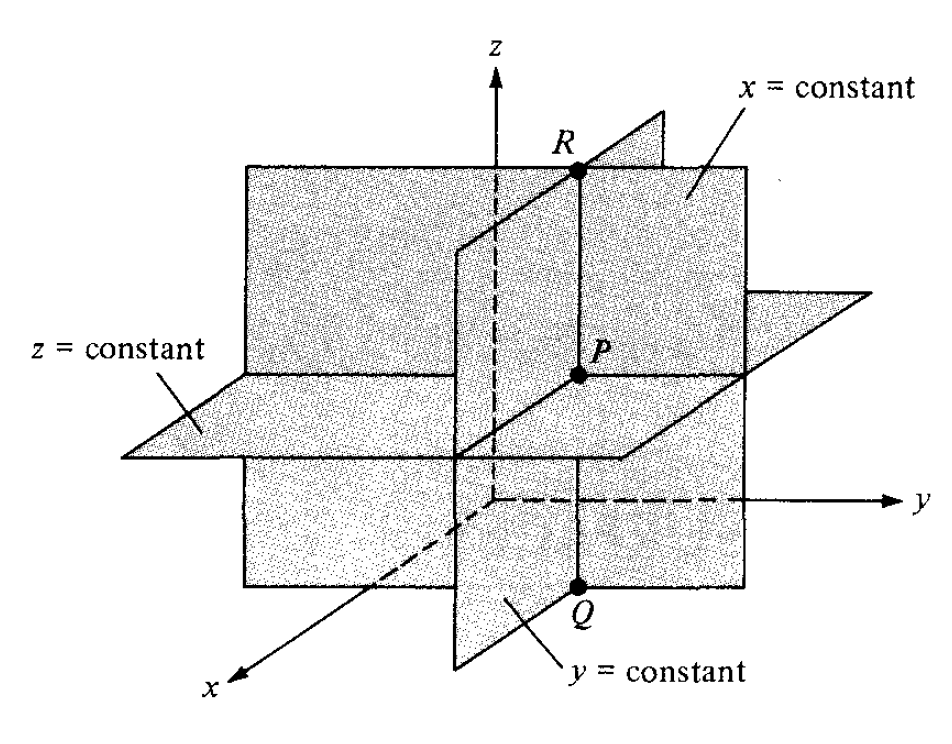
\includegraphics[scale=0.4]{Figure2-7S.png}
\caption{The constant coordinate surfaces in Cartesian coordinates. Figure taken from~\cite[Figure 2.7, page 42]{Sadiku}}
\label{Cartesian-constant}
\end{figure}
\subsection{Cylindrical Coordinates}
In Cylindrical coordinates $\rho=constant$ is a cylindrical surface. $\phi=constant$ is the half plane with one end being $z$--axis. This is illustrated in figure \ref{Cylindrical-constant} taken from~\cite[Figure 2.8, page 43]{Sadiku}.
\begin{figure}[H]
\centering
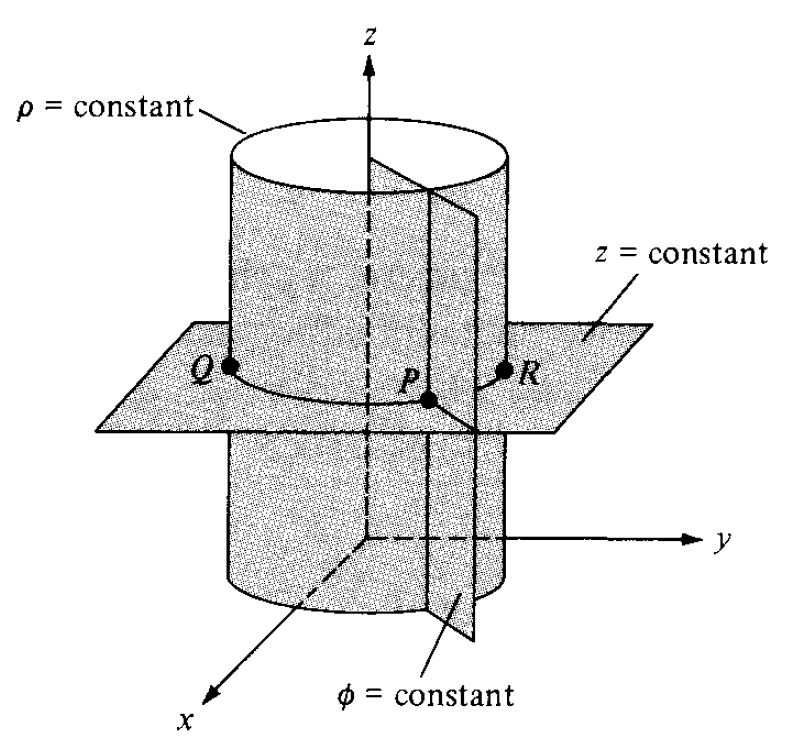
\includegraphics[scale=0.4]{Figure2-8S.png}
\caption{The constant coordinate surfaces in Cylindrical coordinates. Figure taken from~\cite[Figure 2.8, page 43]{Sadiku}}
\label{Cylindrical-constant}
\end{figure}
\subsection{Spherical Coordinates}
In Spherical coordinates $r=constant$ is the surface of a sphere. $\theta=constant$ is a conical surface. This is illustrated in figure \ref{Spherical-constant} taken from~\cite[Figure 2.9, page 43]{Sadiku}.
\begin{figure}[H]
\centering
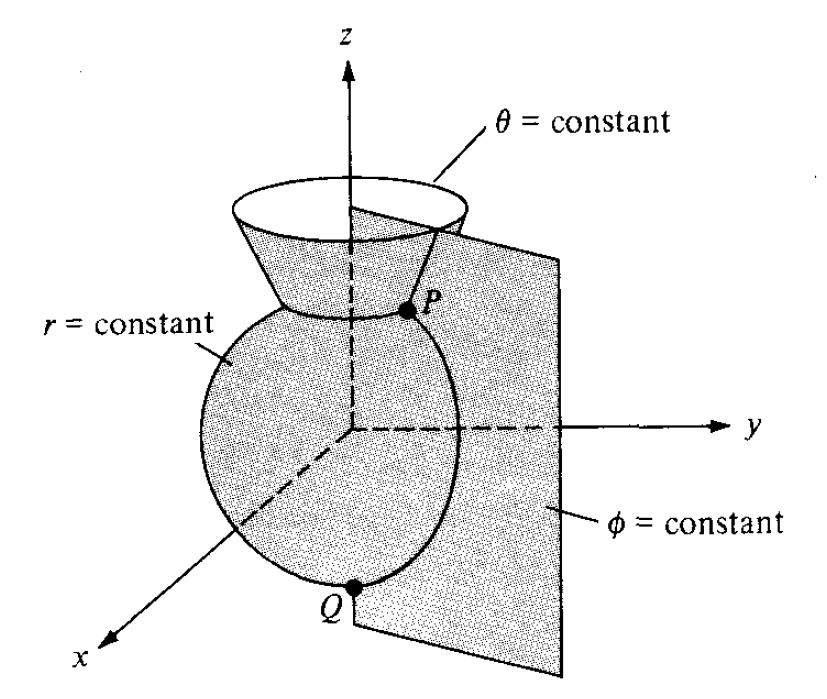
\includegraphics[scale=0.4]{Figure2-9S.png}
\caption{The constant coordinate surfaces in Spherical coordinates. Figure taken from~\cite[Figure 2.9, page 43]{Sadiku}}
\label{Spherical-constant}
\end{figure}
\section{Unit Vector Transformations Between Cartesian and Cylindrical Coordinates}
A vector \textbf{A} in Cartesian and Cylindrical coordinates is expressed in terms of the respective unit vectors. That is,
\begin{equation}
\textbf{A}=A_x\hat x+A_y+\hat y+A_z\hat z=A_{\rho}\hat \rho+A_{\phi}\hat \phi+A_z\hat z
\end{equation}
An extensive discussion on how vectors transform between different coordinate systems is not a part of this course but here we discuss unit vector transformation between cylindrical and spherical coordinate systems. Please consult the reference book \cite[Chapter 2]{Sadiku} for a detailed discussion on vector transformation.

Suppose we want to express vectors $\hat x$ and $\hat y$ in cylindrical coordinates and vice versa. By referring to figure \ref{Cylindrical-Spherical-transformation} taken from ~\cite[Figure 2.3, page 31]{Sadiku} the transformation are
\begin{equation}
\begin{split}
&\hat x=\cos\phi\hat \rho-\sin\phi \hat \phi\\
&\hat y=\sin\phi\hat \rho+\cos\phi \hat \phi\\
&\hat z=\hat z
\end{split}
\end{equation}
\begin{equation}
\begin{split}
&\hat \rho=\cos\phi\hat x+\sin\phi \hat y\\
&\hat \phi=-\sin\phi\hat x+\cos\phi \hat y\\
&\hat z=\hat z
\end{split}
\end{equation}
\begin{figure}[H]
\centering
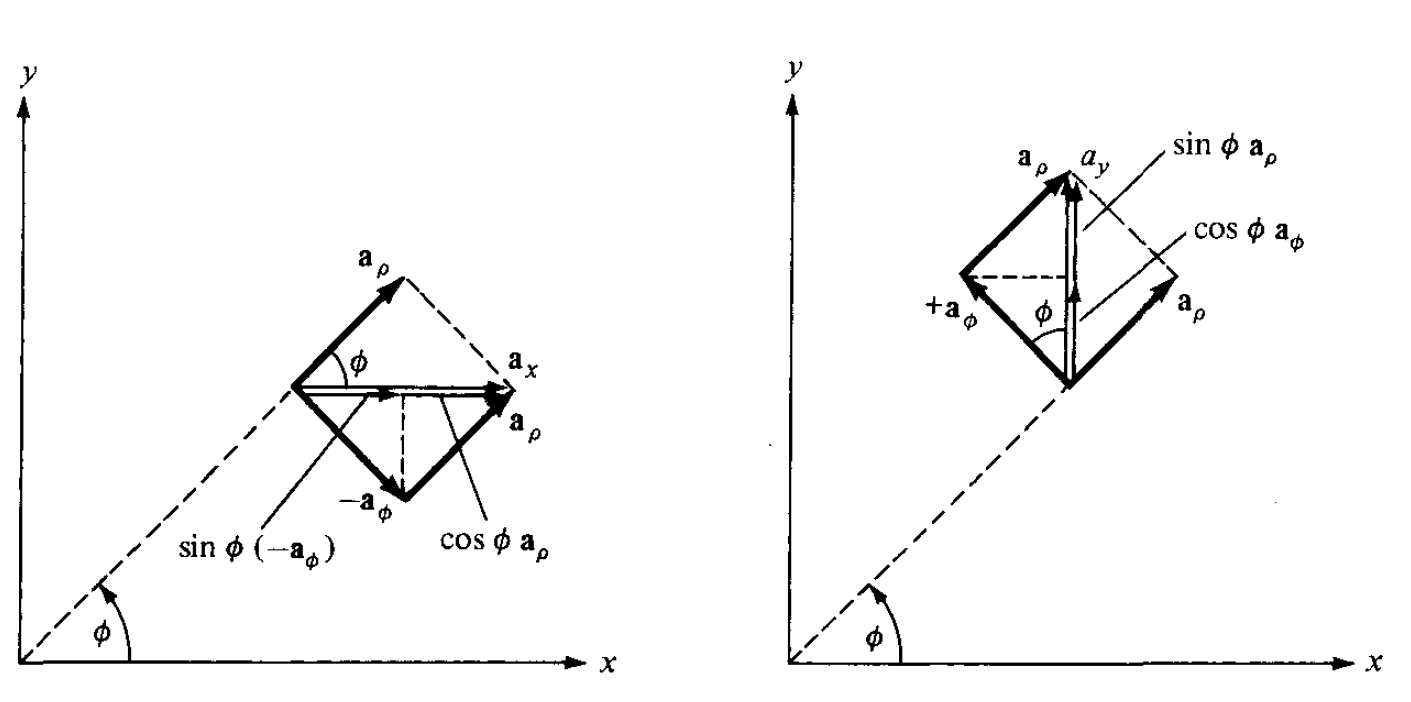
\includegraphics[scale=0.4]{Figure2-3S.png}
\caption{The constant coordinate surfaces in Spherical coordinates. Figure taken from~\cite[Figure 2.3, page 31]{Sadiku}}
\label{Cylindrical-Spherical-transformation}
\end{figure}
\section{Exercises}
\noindent\textbf{Question 1 (PE 2.3S):} Given a vector field in cylindrical coordinates, $\textbf{H}=\rho z\cos\phi\hat\rho+e^{-2}\sin\dfrac{\phi}{2}\hat phi+\rho^2\hat z$, find
\begin{itemize}
\item[(1)] The vector components of \textbf{H} parallel and normal (perpendicular) to $\rho=1$.
\item[(2)] The vector components of \textbf{H} parallel and normal to $z=0$ plane.
\end{itemize}
%\nocite{*}
\bibliographystyle{plain}
\bibliography{PhysicsRef}
\end{document}
